\chapter{\label{ch:3-polycubes}Modular self-assembly of polycubes}

\minitoc

As introduced in the previous chapter, there is an increasing interest within the field of DNA nanotechnology to create finite-sized multi-component objects. While some coarse-grained tile models exists, there still remains a need for methods to quickly explore the assembly of multi-component 3D structures.
This chapter describes my polycube model and details how it can be used to sample a large amount of assembly rules, showing that some polycube shapes are significantly more common than others. The following chapter will show how to obtain the simplest assembly rule for any given polycube shape.

\section{The polycube model}
A polycube consists of a number of equally-sized cubes, connected by their neigbouring faces; a three-dimensional analogue to how polyominos are squares connected by their neigbouring edges. In the model presented here, a polycube is stochastically self-assembled according to a specified rule, where a rule is a set of available species. Each cube species describes a type of cube that can be present in the polycube; cubes belonging to the same species are always identical.

Each species has six patches; one on each face of the cube, and each patch has a "colour" and an orientation. The colour is indicated by a signed integer and the orientation is one of four possible rotations: 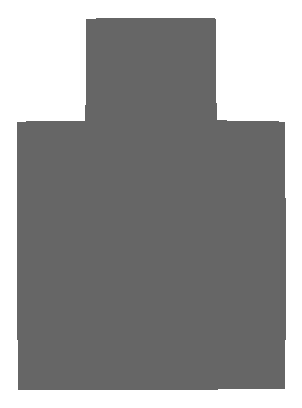
\includegraphics[width=10pt]{figures/face.eps}\hspace{4pt}(\(0\)),
\begingroup\setbox0=\hbox{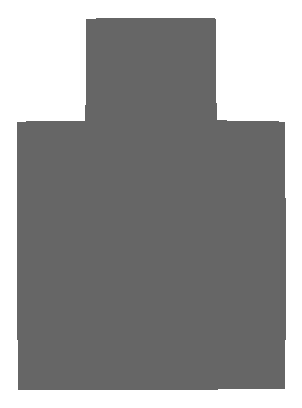
\includegraphics[width=10pt,angle=-90]{figures/face.eps}}\parbox{\wd0}{\box0}\endgroup\hspace{4pt}(\(\frac{\pi}{2}\)),
\begingroup\setbox0=\hbox{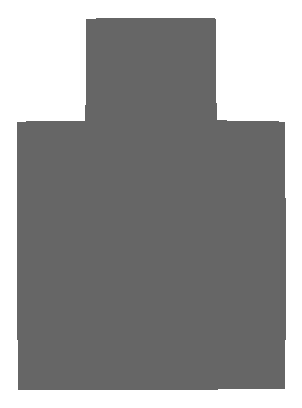
\includegraphics[width=10pt,angle=180]{figures/face.eps}}\parbox{\wd0}{\box0}\endgroup\hspace{4pt}(\(\pi\)) or
\begingroup\setbox0=\hbox{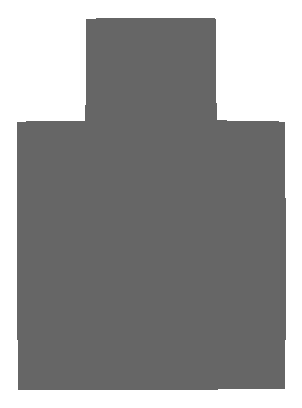
\includegraphics[width=10pt,angle=90]{figures/face.eps}}\parbox{\wd0}{\box0}\endgroup\hspace{4pt}(\(\frac{3\pi}{2}\)). A patch can bind to another patch if and only if they have the opposite colour and the same orientation. If the patch color is zero, the patch is considered empty and will not bind to anything. The model can also be expanded to more complicated colour interaction matrices or changed to pair odd integers with each subsequent integer as in the polyomino model\cite{ahnert2010self}\cite{johnston2011evolutionary} described in Section \ref{sec:polyomino}.

The stochastic self-assembly of a polycube starts by placing a cube from one of the available species as a seed at the origin. If the assembly mode is set to be seeded, it will always use first species in of rule. If the assembly mode is stochastic, the species of the seed is chosen at random.

Each possible neighbour to the placed cube, given the cube's patches, is then added to a list of possible moves. For the next step, a possible move is chosen at random and the rule is searched in a random order for a species fitting the move. Cubes can be rotated to fit and if a fitting species is found, the corresponding cube is added. If there is no fit, the move is discarded. Moves are processed until the list of moves is empty or the polycube grows beyond a specified size, at which point it is considered unbounded.

To determine if the rule is deterministic, the assembly is repeated \(n_{times}\) times (default 10) and the outputs compared for equality (allowing rotation).

ADD FIGURE ABOUT DETERMINISTIC AND UNBOUNDED ASSEMBLIES!!

It could be argued, instead of first picking a random move and then randomly trying all available species to find a fit, that one should pick both a move and a species at random until a fit is found. While this would take longer time, it would avoid biasing the assembly toward unlikely assembly results, where a move is picked that would otherwise usually be blocked by more likely surrounding cubes. However, since only deterministic and bounded rules are of interest, this would only affect the end result in the cases where the bias is strong enough and \(n_{times}\) is low enough to falsely make the rule seem deterministic.

\begin{figure}
\centering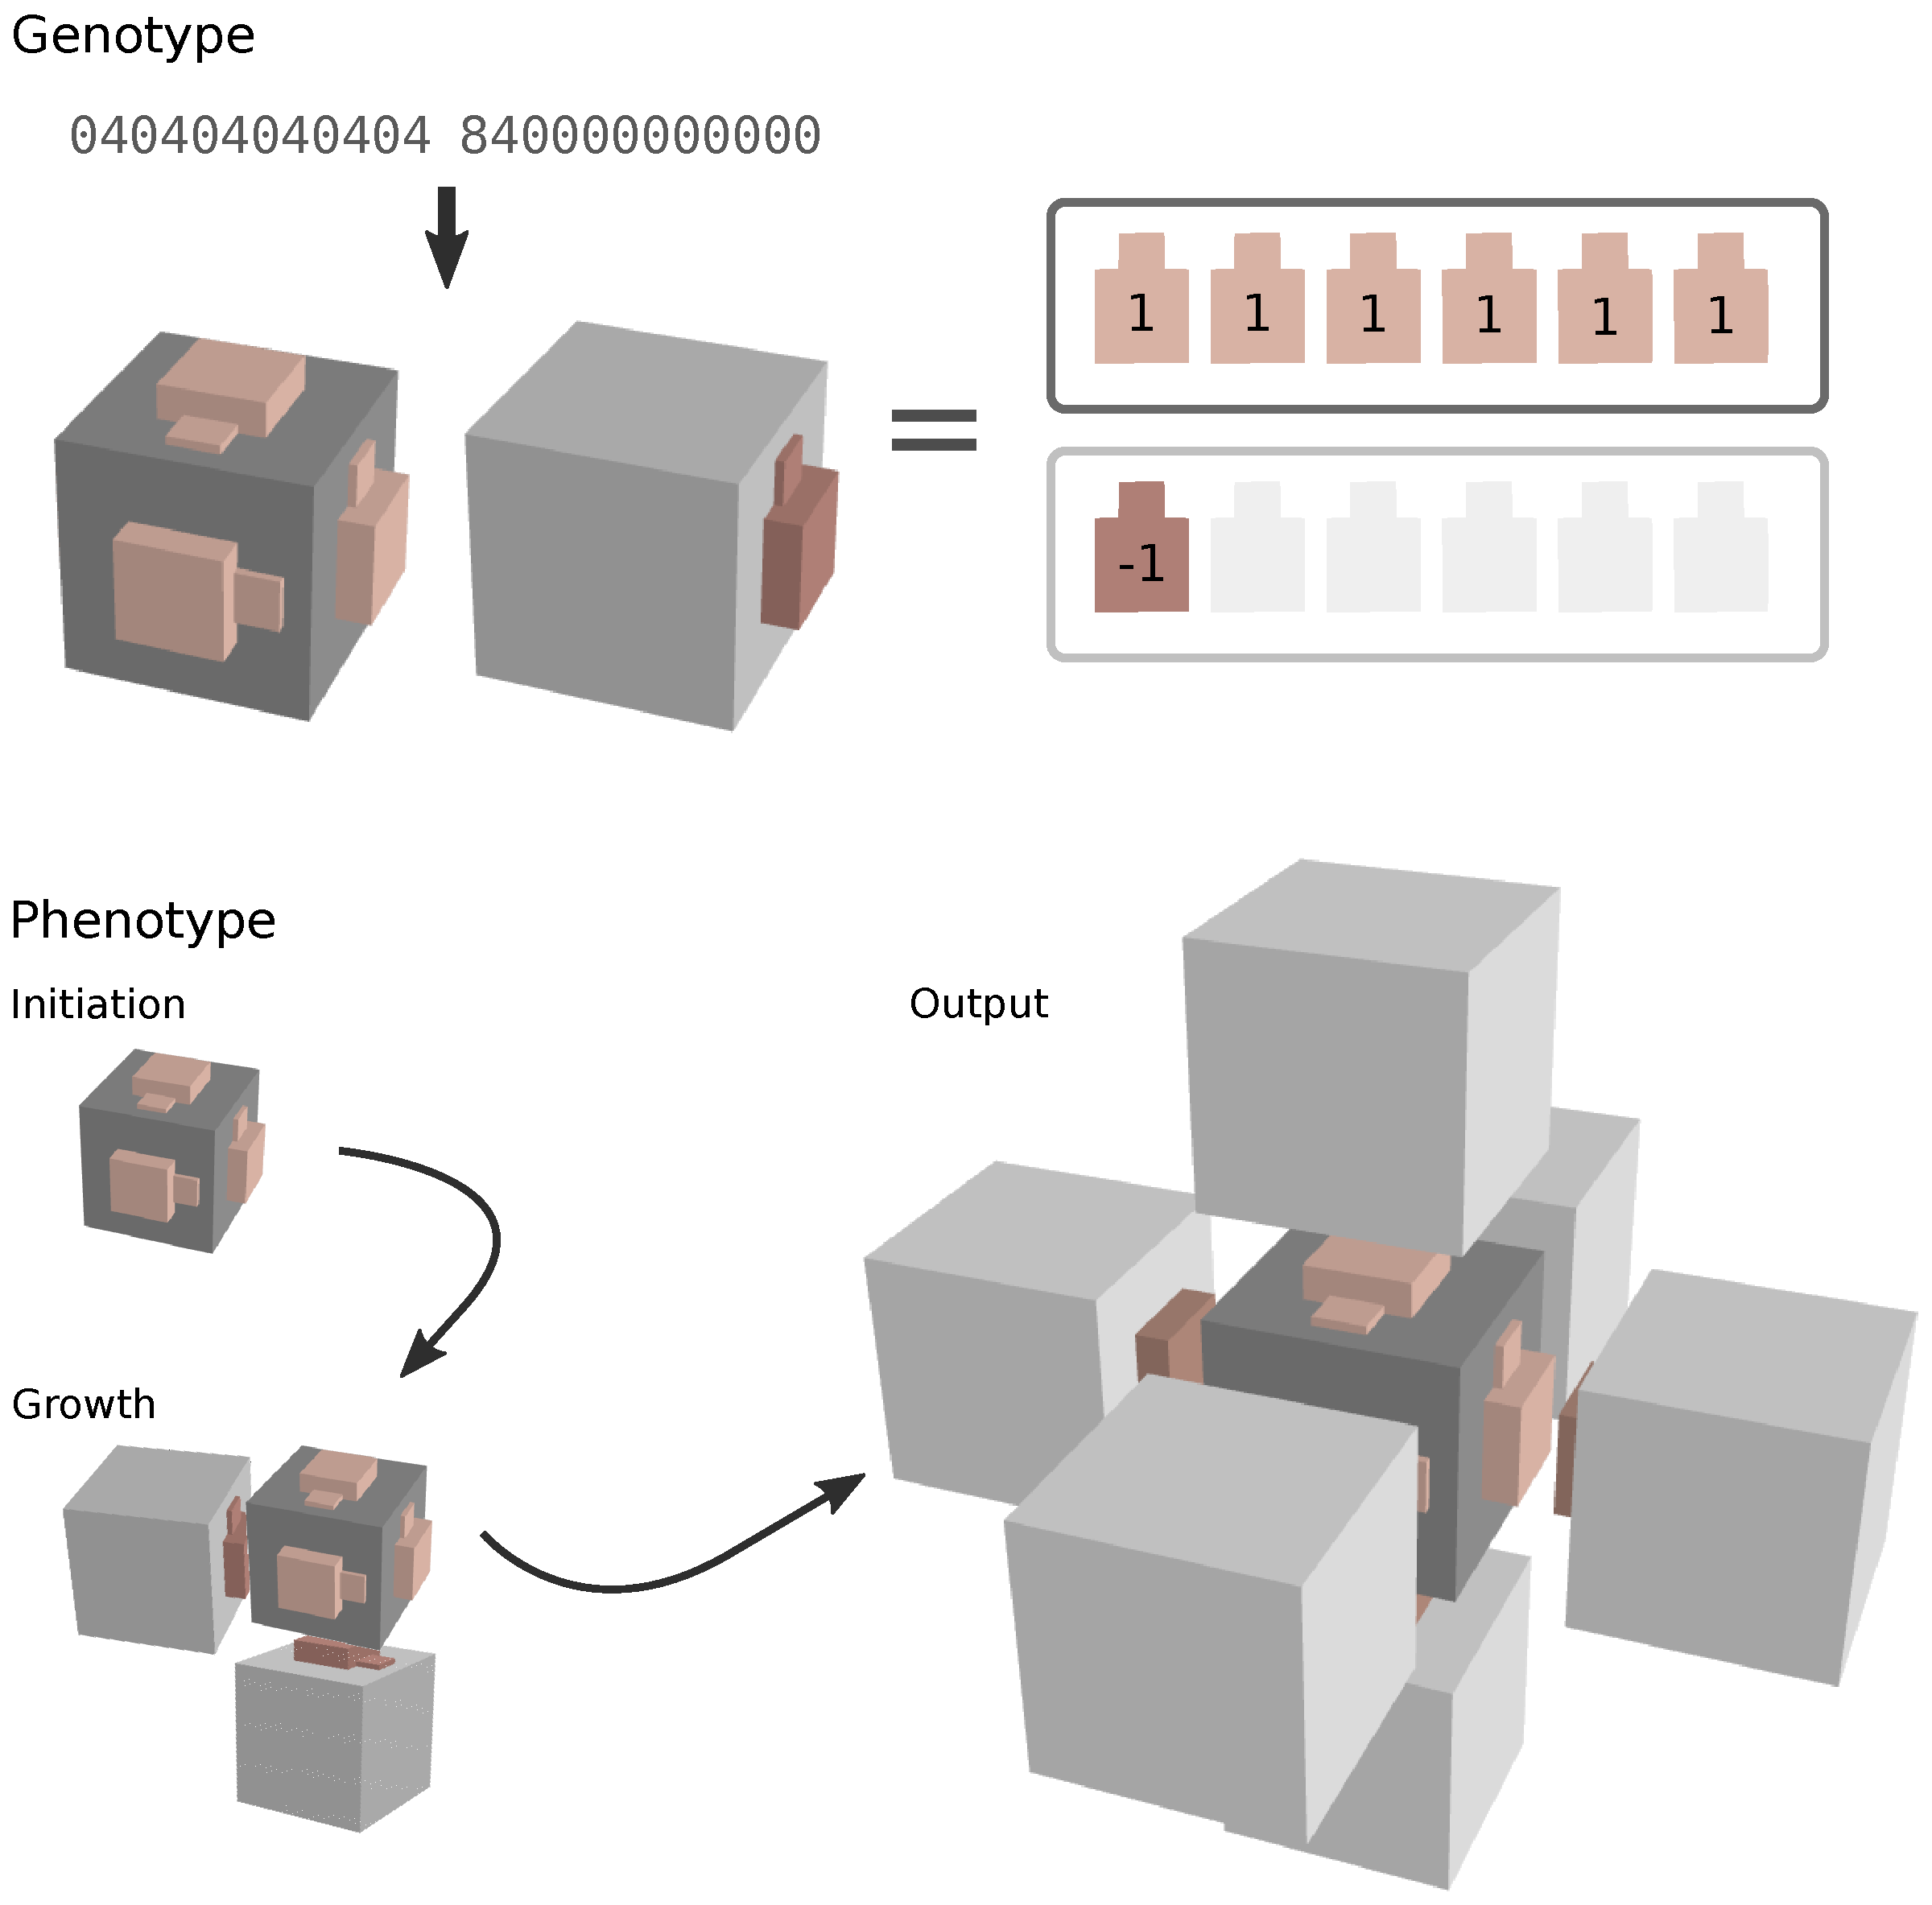
\includegraphics[width=0.8\textwidth]{figures/rule.eps} 
\caption{Illustration of the polycube assembly model. Compare to the polyomino model in Figure \ref{fig:polyominoes}. The top of the figure shows the genotype, in the form of a rule with two species one colour. The rule is visualised in three different ways. The first is a hexadecimal representations, with each two digits coding for a patch and a total of 12 digits describing a species. The second representation is of the two species shown as 3D cubes. The first species has colour=1 on all patches while the second has a single patch with colour=-1. Since the polycube is symmetric the patch rotations do not matter and are all kept at 0.}
\label{fig:polycubeRule}\end{figure}

For an illustration of the model, see Figure \ref{fig:polycubeRule}. The example in the figure is a three-dimensional "cross" structure created from a rule of size 2. The initial seeding cube belongs to the first species, enabling six additional cubes, all belonging to the second species, to bind at each patch. They bounds are made since the patch colours \(1\) and\( -1\) are opposites. After all six outer cubes have bound, there are no remaining possible moves and thus the polycube stops growing. Since the growth stops, this particular polycube is bounded, at a size of seven cubes. Furthermore, since the rule gives the same polycube every time it is evaluated, the polycube is deterministic.

\begin{figure}
    \centering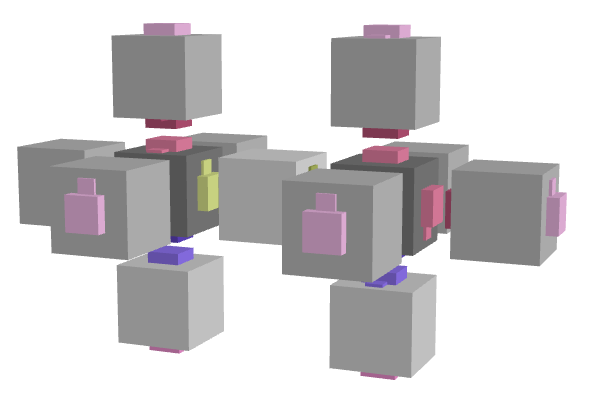
\includegraphics[align=c,width=0.24\textwidth]{figures/dnaRoboticPolycubes/doubleplus.png}\hfill
    \centering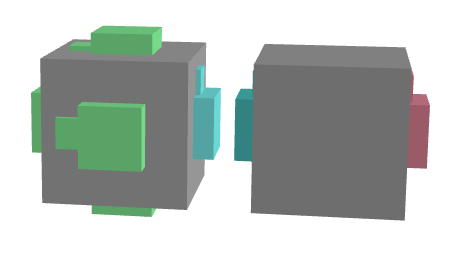
\includegraphics[align=c,width=0.24\textwidth]{figures/dnaRoboticPolycubes/swimmer.png}\hfill
    \centering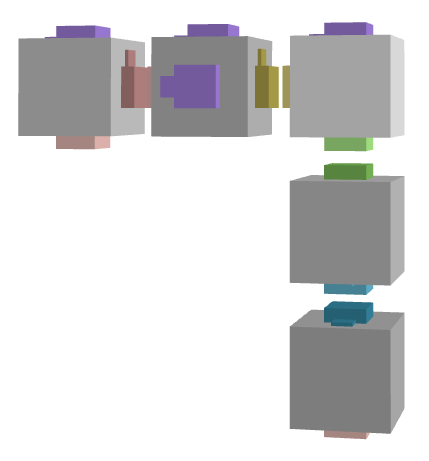
\includegraphics[align=c,width=0.24\textwidth]{figures/dnaRoboticPolycubes/L.png}\hfill
    \centering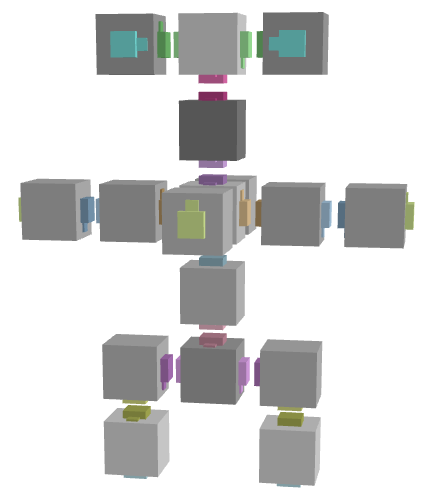
\includegraphics[align=c,width=0.24\textwidth]{figures/dnaRoboticPolycubes/robot.png}
\caption{Polycube versions of the conceptual DNA Robotics designs. Compare to Figure \ref{fig:dnaRoboticsHeader}. From left to right, the size of the rule required to specify each polyomino is: \href{https://akodiat.github.io/polycubes/view?hexRule=040890040707840c00000000888a00000000101400000000}{\underline{4}}, \href{https://akodiat.github.io/polycubes/view?hexRule=0a040b0b080a840e00000000}{\underline{2}}, \href{https://akodiat.github.io/polycubes/view?hexRule=06000c0b00001284000b080a0090140b00000000188c0000000014980000}{\underline{5}} and \href{https://akodiat.github.io/polycubes/view?hexRule=0406008800008400240000008c0800000000903400000000980c2f2f10129c1a0000000094000000002214141c000000000028a40000ac3200000000b43000000000}{\underline{11}}. Note how the third polyomino (L-shaped) requires a larger rule than the first (double cross), although it is smaller in size. This is because each cube in the L-shaped nanobot needs to be unique, while the double-cross-shaped first nanobot consists of two identical parts. If we only wished to reproduce the polycube shape, the rulesets could be minimised further.}
\label{fig:dnaRoboticPolycubes}\end{figure}

The polycube assembly model has been implemented in two versions: one browser implementation for outreach activities and accessible visualisation, and one C++ implementation for fast rule evaluation. Using the C++ implementation, large sets of random rules have been evaluated and the resulting polycubes examined and categorised. This has also been repeated for different values of rule size and colour limits.

See figure \ref{fig:rs_vs_ps} for a heat map of the frequency of rules of a certain size creating polycubes of a certain size. Notice how only three different polycube sizes were found for one species. This is understandable when inspecting the first column in Figure \ref{fig:poly_examples}; using only one species, you cannot create a bounded structure of any other size.

For larger rule sizes, polycubes can have any form, as shown in Figure \ref{fig:dnaRoboticPolycubes}, but upon inspection of the larger polycube sizes (and small rule sizes) from Figure \ref{fig:rs_vs_ps}, the polycubes all seem to be highly symmetrical, as shown in \ref{fig:poly_examples}.
%I have already implemented a fast version of the code that can generate random rules with a certain max amount of "colours" and tile types. The next step is to determine what (deterministic) structures are more common. (Rules creating non-deterministic structures are disregarded, but their percentage of the total is still noted). Plotting the probability of each structure, from a random rule, against a measure of its complexity, do we get a power-law distribution (as in Iain Johnston's polyomino paper)?


\begin{figure}
\centering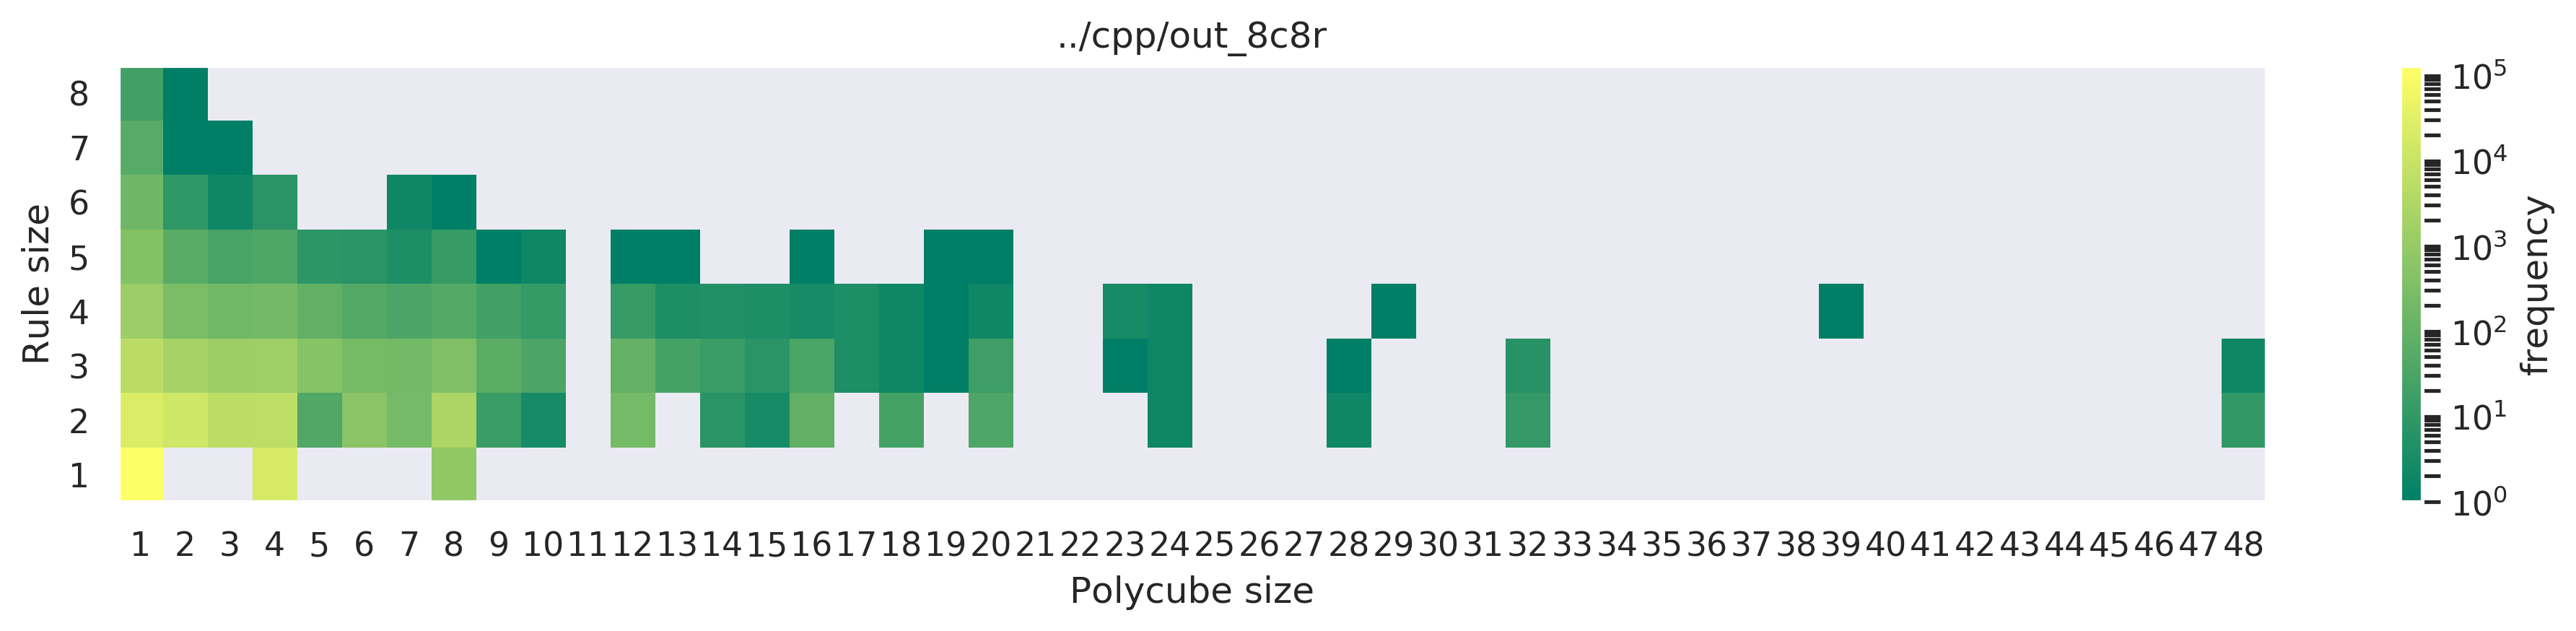
\includegraphics[width=\textwidth]{figures/rs_vs_ps_8c8r.png}
\caption{Heat map of rule size vs polycube size, for a simulation with a maximum of 8 species and a limit of 8 colours, evaluating 2.5 million random rules. Note that the frequency scale is logarithmic.}
\label{fig:rs_vs_ps}\end{figure}

\begin{figure}
%\centering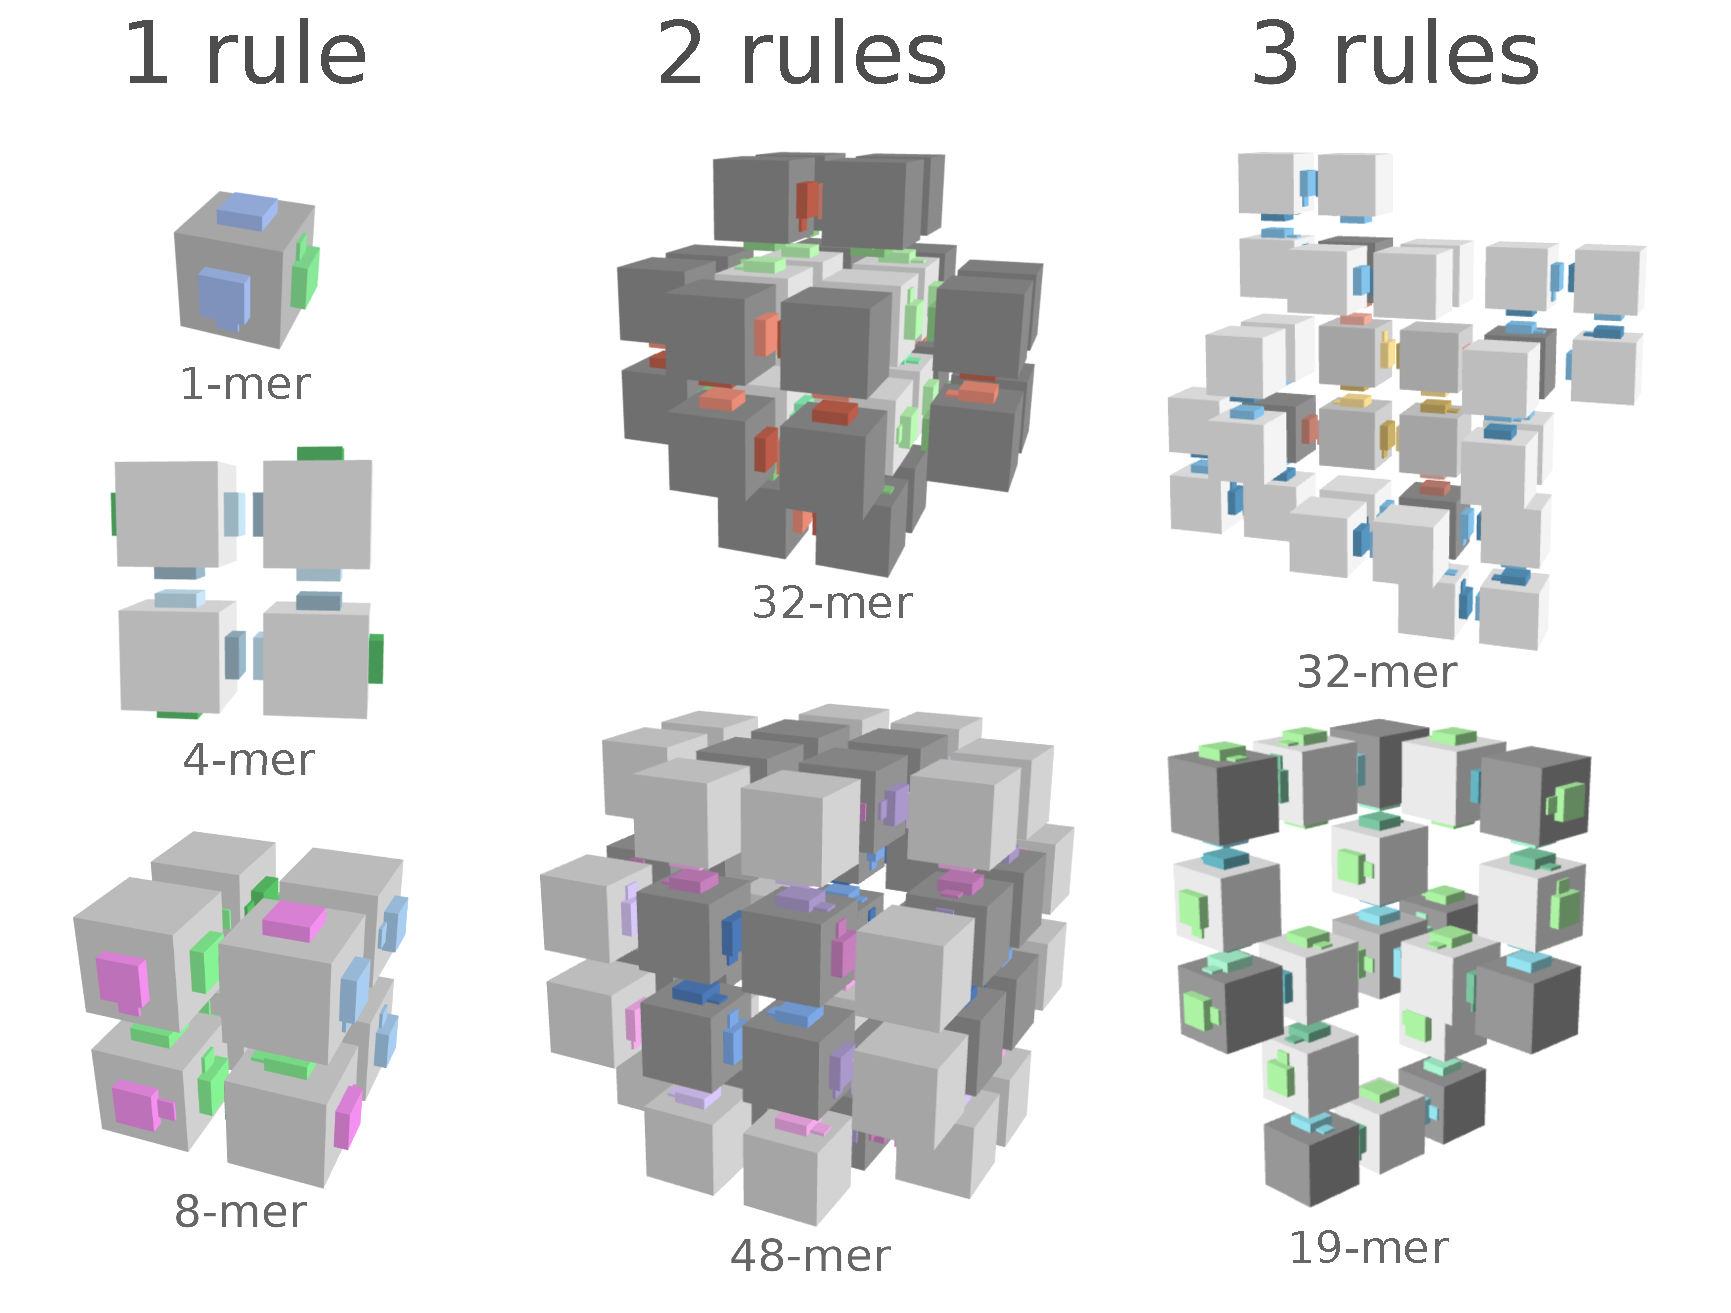
\includegraphics[width=\textwidth]{figures/examples.eps}
\caption{Example of polycubes grown from 1, 2 and 3 speciess. Although any polycube can be encoded into a rule, the larger polycubes that have small rules tend to be symmetrical. This agrees with Johnston's polyomino model in that they have low complexity}
\label{fig:poly_examples}\end{figure}

\section{Sampling the space of assembly rules}

\[
I_{n_c, n_t} = (4(1+2n_c))^{6n_t}
\]

Trying all inputs in a brute-force approach is impossible. Even if we limit both the amount of allowed colours \(n_c\) and the amount of species \(n_t\) to eight, the space of possible inputs, with four patch orientations and six patches per cube, is \(I_{8, 8} \approx 9*10^{87}\).
But, while this is too large to sample fully, we can still get an idea of how likely it is for an input to map to a certain output by taking samples of the space of possible input rules.

This was done by uniformly sampling and assembling one billion random rules from \(I_{8, 8}\). Rules growing larger than 100 cubes were discarded as unbounded, while those remaining bounded were re-assembled 15 times to ensure they assembled deterministically. Deterministic and bounded output was then grouped by their shapes, counting the number of times each given phenotype occurs. For each rule found to produce a given phenotype, the number of colours is multiplied with the number of species in the rule, producing a measure of the rule size. The smallest such rule size is then used as a proxy for the phenotype complexity.

\section{Complexity bias}

As can be seen in Figure \ref{fig:plot}, there is a clear log-linear relationship between the probability of finding a rule that assembles into a particular structure, and the information needed to specify the structure, as predicted in \cite{dingle2018input, dingle2020generic}.

\section{Robustness}
